\section{Auswertung}
\label{sec:Auswertung}

Im Folgenden werden alle Berechnungen in Python 3.7.1, unterstützt durch das
Paket NumPy \cite{numpy}, durchgeführt. Die Abbildungen werden mit matplotlib \cite{matplotlib} erstellt.

(VIELLEICHT NOCH ERKLÄREN WAS GENAU JETZT HIER MIT DEM FEHLER IST UND WIESO DER NICHT EINFACH DIE WURZEL IST)

\subsection{Untersuchung des Spektrums}

Das Spektrum der Quelle ist in Abbildung \ref{fig:spektrum} dargestellt. Dort ist die Anzahl der gemessenen Ereignisse gegen die Nummer des channels, in dem sich die Eregnisse befinden, aufgetragen.

\begin{figure}
  \centering
  \includegraphics[width=\textwidth]{build/spektrum.pdf}
  \caption{Spektrum der Caesium-Quelle.}
  \label{fig:spektrum}
\end{figure}

Bei der Betrachtung von links nach rechts sind im Spektrum zunächst beim ersten
Maximum die Rückstreulinie, danach das Compton-Kontinuum, daraufhin beim zweiten
Maximum die maximale Compton-Energie und anschließend den Photopeak.

Die Rückstreulinie entsteht dadurch, dass der Strahler in alle Richtungen strahlt und auch an den Bleiwänden Compton-gestreute Photonen in den Detektor gelangen können. Das Compton-Kontinuum entsteht durch die Wechselwirkung der Gammaphotonen mit dem Szintillationsdetektor, wobei sie unter einem bestimmten Winkel gestreut werden und dabei Energie abgeben. Dieser Effekt findet nur bis zu einer bestimmten Energie statt, sodass eine maximale Compton-Energie zu erkennen ist.
Der Photopeak repräsentiert schließlich die tatsächliche Energie der Gammaphotonen
und beträgt
\begin{equation*}
  E=\SI{661.7}{\kilo\eV} \,.
\end{equation*}
Die Zählrate für die Nullmessung kann zu
\begin{equation*}
  I_0=\SI{184.08(87)}{\per \second}
\end{equation*}
bestimmt werden.

(ZITAT)

\subsection{Untersuchung eines leeren Aluminiumgehäuses}

Zur Untersuchung des leeren Aluminiumgehäuses wurden für die in Abbildung \ref{fig:wuerfel1} dargestellten Projektionen die Zählraten gemessen.

\begin{figure}
  \centering
  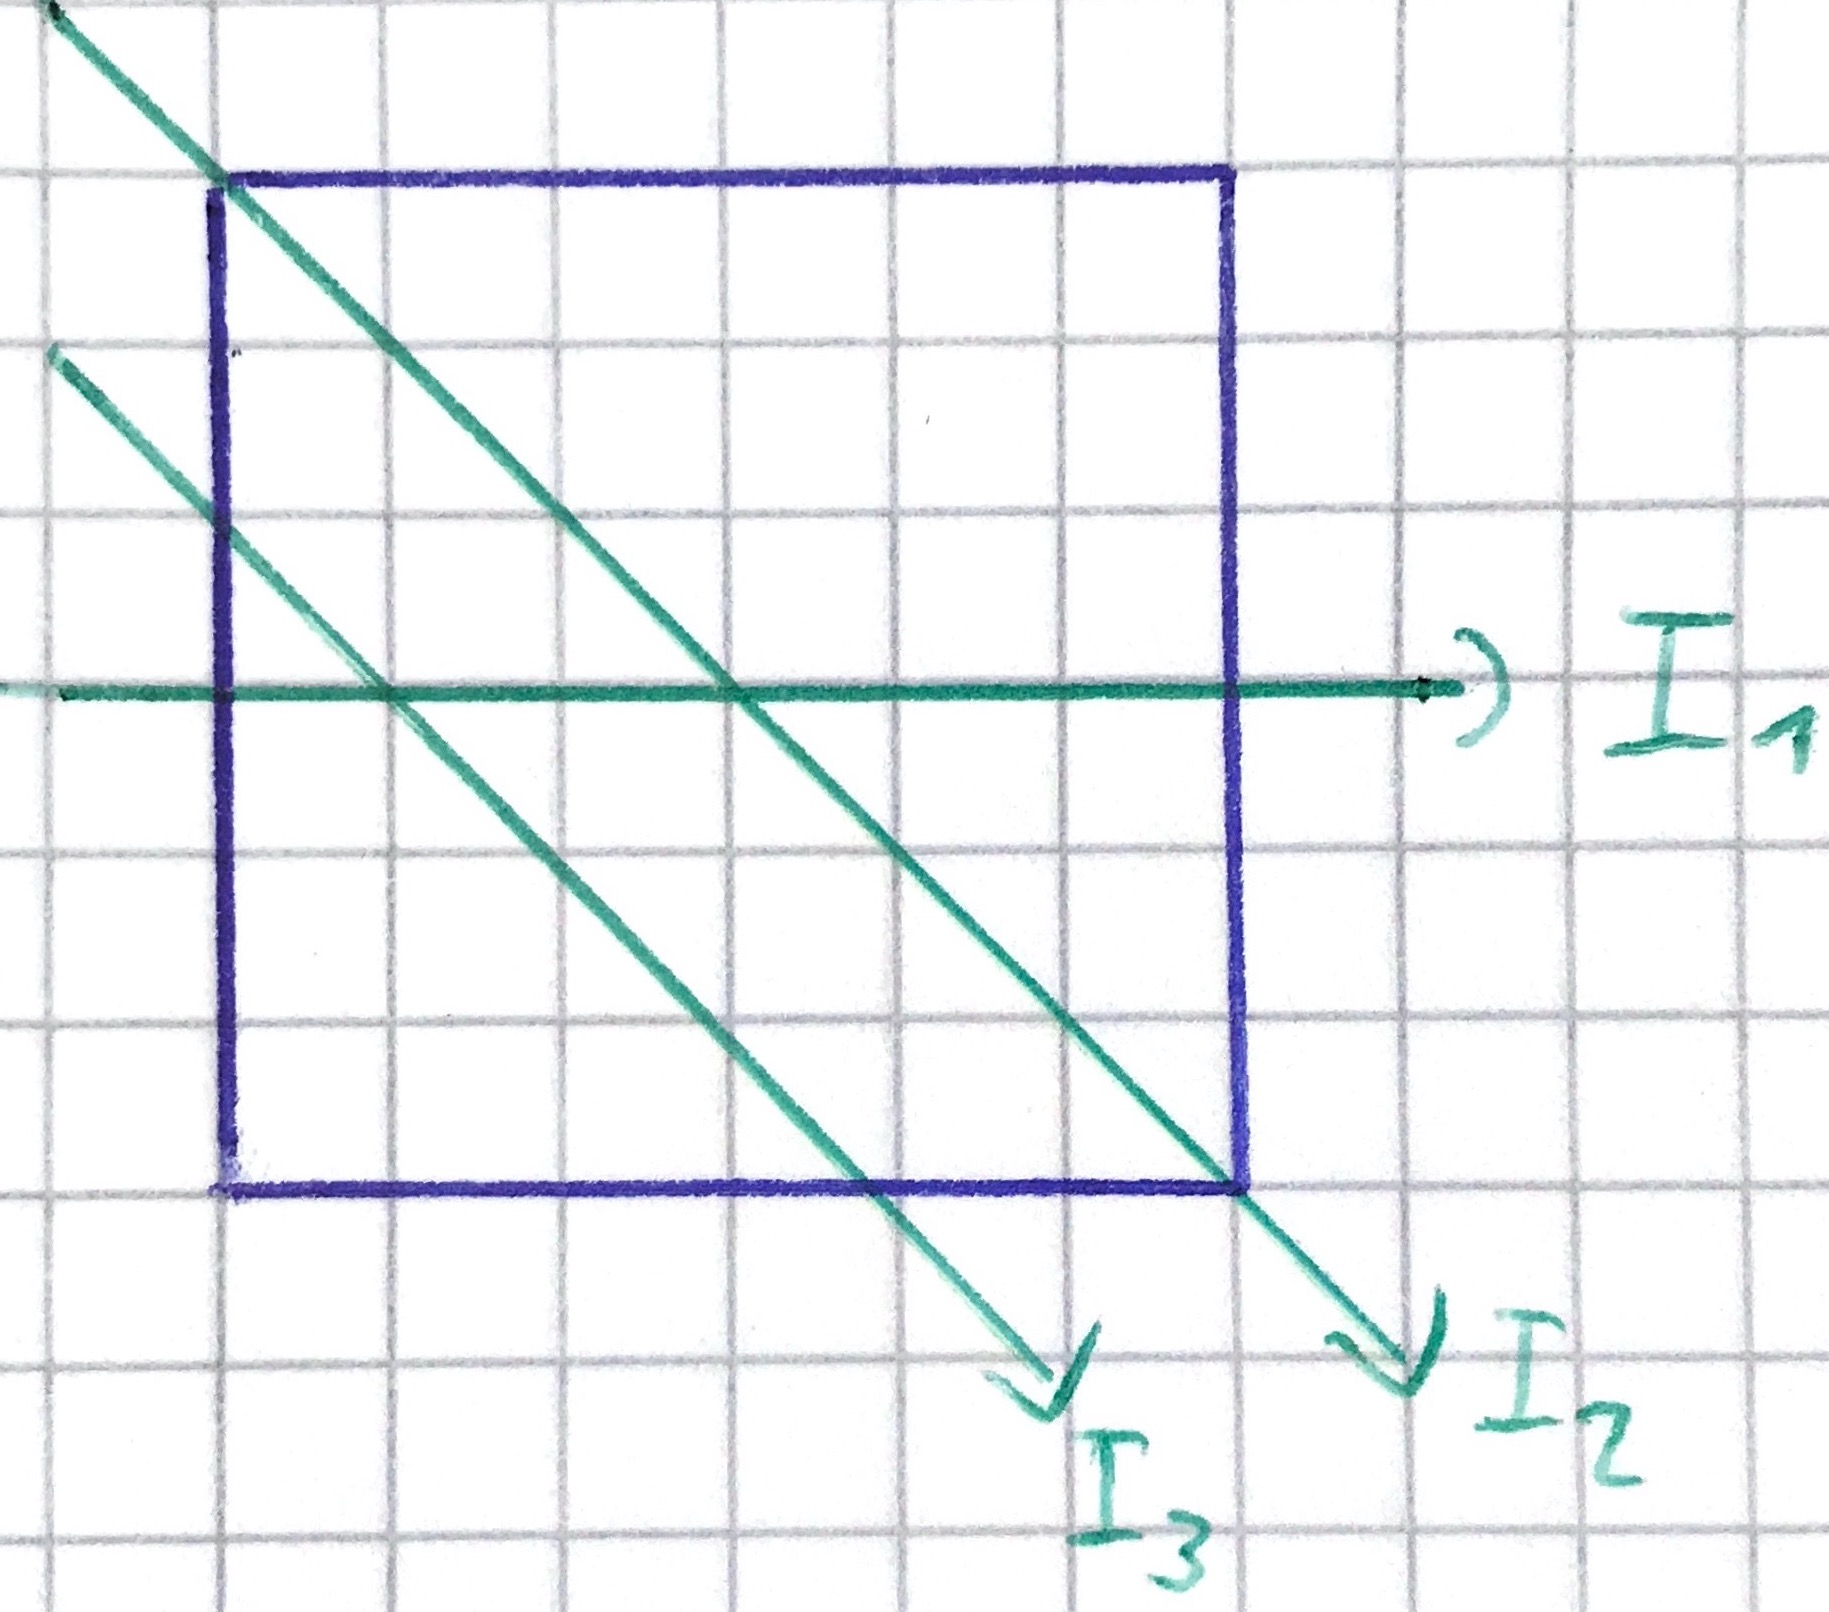
\includegraphics[width=0.5\textwidth]{images/wuerfel1.jpg}
  \caption{Skizze der gemessenen Projektionen für das reinen Aluminiumgehäuse.}
  \label{fig:wuerfel1}
\end{figure}

Da alle folgenden Würfel ebenfalls ein Aluminiumgehäuse besitzen und die Absorption durch das Aluminiumgehäuse somit bei jedem Würfel auftritt, werden
diese Messungen als Nullmessungen für den jeweiligen Projektionstyp gewählt. Das bedeutet $I_{0,1}$ ist die Nullmessung für gerade Projektionen,  $I_{0,2}$ ist die Nullmessung für diagonale Projektionen durch eine Hauptdiagonale des Würfels
und $I_{0,3}$ ist die Nullmessung für diagonale Messungen durch eine Nebendiagonale des Würfels.

Es ergeben sich die Zählraten
\begin{align*}
  I_0,1&=\SI{171.83(135)}{\per\second} \,, \\
  I_0,2&=\SI{169.63(133)}{\per\second} \,, \\
  I_0,3&=\SI{158.78(133)}{\per\second} \,.
\end{align*}

\subsection{Bestimmung des Materials zweier homogener Würfel}
Zur Bestimmung des Materials zweier homogener Würfel werden die Zählraten für die
in Abbildung \ref{fig:wuerfel2} dargestellten Projektionen gemessen. Die gemessenen Werte befinden sich in Tabelle \ref{tab:wuerfel2}.

\begin{figure}
  \centering
  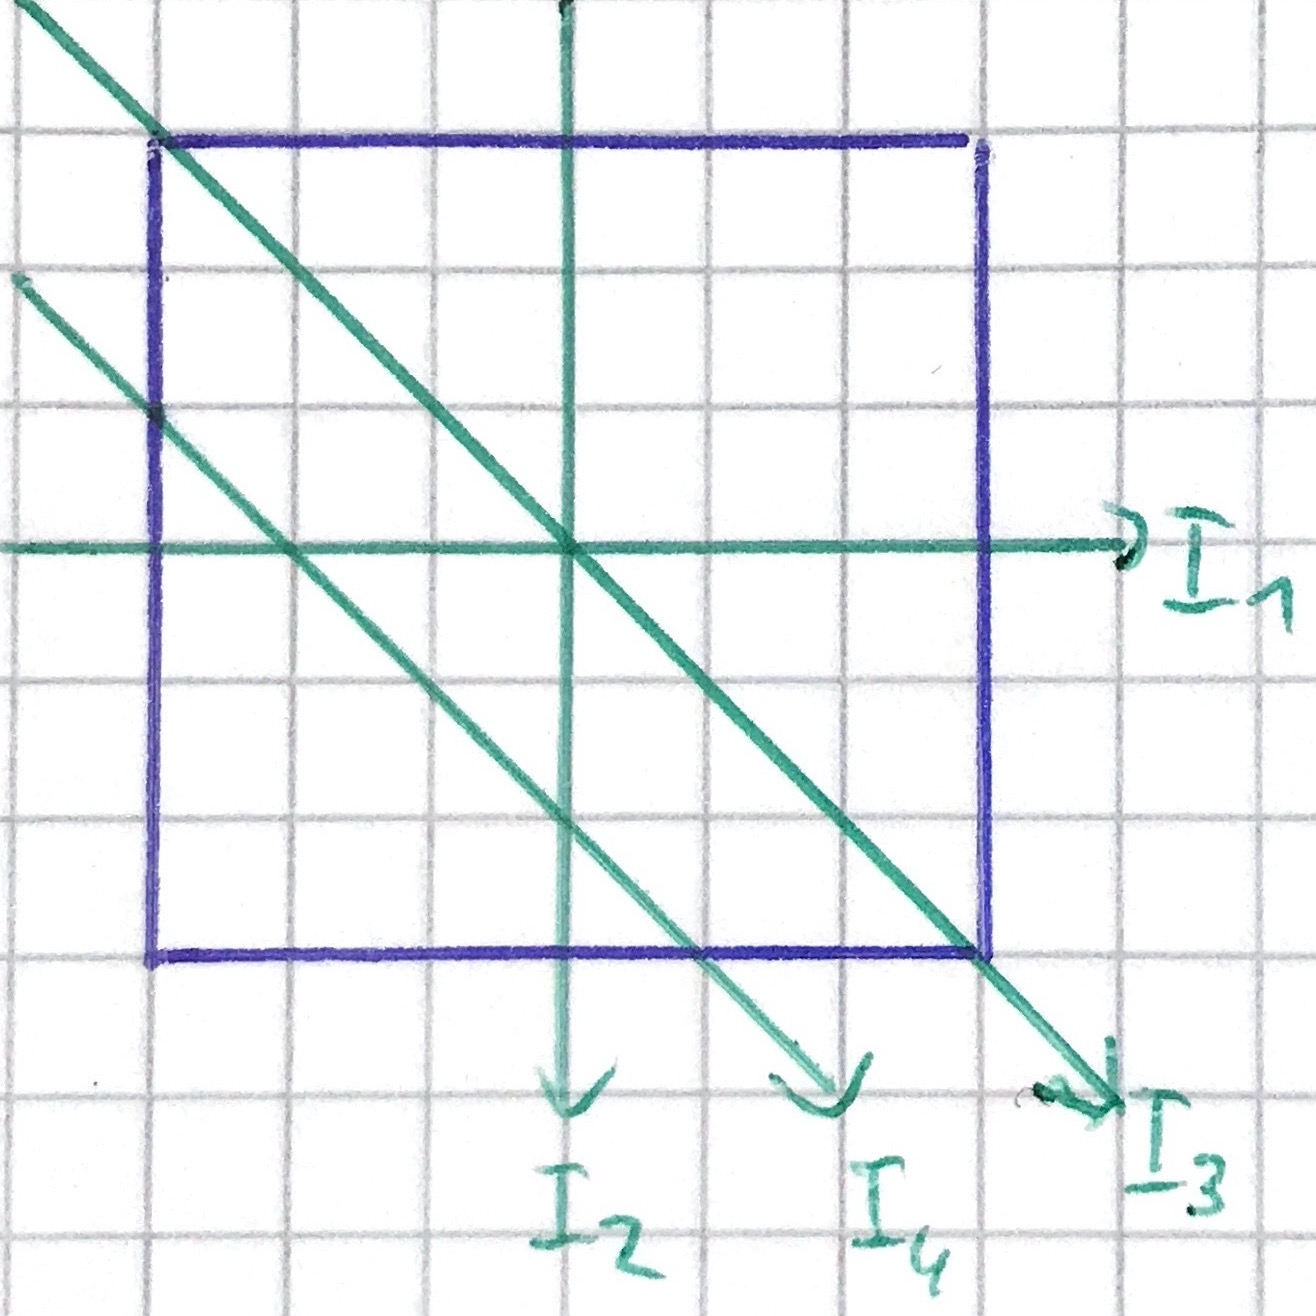
\includegraphics[width=0.5\textwidth]{images/wuerfel2.jpg}
  \caption{Skizze der gemessenen Projektionen für die homogenen Würfel.}
  \label{fig:wuerfel2}
\end{figure}

\begin{table}[htp]
	\begin{center}
    \caption{Messwerte und daraus berechnete Zählraten für die beiden homogenen Würfel.}
    \label{tab:wuerfel2}
		\begin{tabular}{ccccc}
		\toprule
			{Projektion} & {$N_2$}  & {$I_2$/(1/s)}  & {$N_3$}  & {$I_3$/(1/s)}\\
			\midrule
			1 & 4981 \pm 80 & 27,67 \pm 0,44 & 20566 \pm 165 & 114,26 \pm 0,92\\
			2 & 4594 \pm 81 & 25,52 \pm 0,45 & 20670 \pm 167 & 114,83 \pm 0,93\\
			3 & 2906 \pm 62 & 16,14 \pm 0,34 & 17772 \pm 159 & 98,73  \pm 0,88\\
			4 & 4464 \pm 77 & 24,80 \pm 0,43 & 19603 \pm 166 & 108,91 \pm 0,92\\
		\bottomrule
		\end{tabular}
	\end{center}
\end{table}

Aus den gemessenen Zählraten kann der Absorptionskoeffizient über den Zusammenhang
\begin{equation}
  \mu_i=\frac{1}{l_i} \ln \left(\frac{I_{0,j}}{I_i} \right)
\end{equation}
bestimmt werden. Dabei ist $l_i$ die Strecke, die die Gammastrahlung durch den Würfel zurücklegt, $I_{0,j}$ die Nullzählrate für die entsprechende Art der Projektion und $I_i$ die Zählrate für die Projektion durch den Würfel. Der zugehörige Fehler kann mithilfe der Gauß'schen Fehlerfortpflanzung zu
\begin{equation}
  einguegen
\end{equation}
bestimmt werden. Die Ergebnisse sind in Tabelle \ref{tab:ergebnisse} dargestellt.

\begin{table}[htp]
	\begin{center}
    \caption{Berechnete Werte für die Absorptionskoeffizienten}
    \label{tab:ergebnisse}
		\begin{tabular}{ccccc}
		\toprule
		{Projektion} &{$\mu_2$/(1/cm)} & {$\mu_3$/(1/cm)}\\
			\midrule
			1 & 0,609 \pm 0,006 & 0,136 \pm 0,006\\
			2 & 0,636 \pm 0,006 & 0,134 \pm 0,006\\
			3 & 0,554 \pm 0,005 & 0,128 \pm 0,005\\
			4 & 0,656 \pm 0,007 & 0,133 \pm 0,007\\
		\bottomrule
		\end{tabular}
	\end{center}
\end{table}

Die Einzelergebnisse werden noch mit
\begin{align}
  \bar{\mu}&= \frac{1}{4} \sum_{i=1}^4 \mu_i \, 
  %\Delta\bar{\mu}&=\sqrt{\frac{1}{12} \sum_{i=1}^4 (\bar{\mu}-\mu_i)^2}
\end{align}
gemittelt. Damit folgt für die gemittelten Absorptionskoeffizienten
\begin{align*}
  \bar{\mu_2}&= \SI{0.614(42)}{1\per \centi\metre}\,, \\
  \bar{\mu_3}&=\SI{0.133(9)}{1\per \centi\metre} \,.
\end{align*}
Damit können den Würfeln die Materialien Messing für Würfel 2 und
CH2O für Würfel 3 zugeordnet werden. Die Abweichungen von den Literaturwerten
betragen $1{,}57\%$ und $14{,}75\%$.

\subsection{Bestimmung der Materialien in einem zusammengesetzten Würfel}

Für den aus verschiedenen Materialien zusammengesetzten Würfel werden die Zählraten für die in Abbildung \ref{fig:wuerfel4} dargestellten Projektionen
gemessen. Die gemessenen Werte sind in Tabelle \ref{tab:wuerfel4} aufgeführt.

\begin{figure}
  \centering
  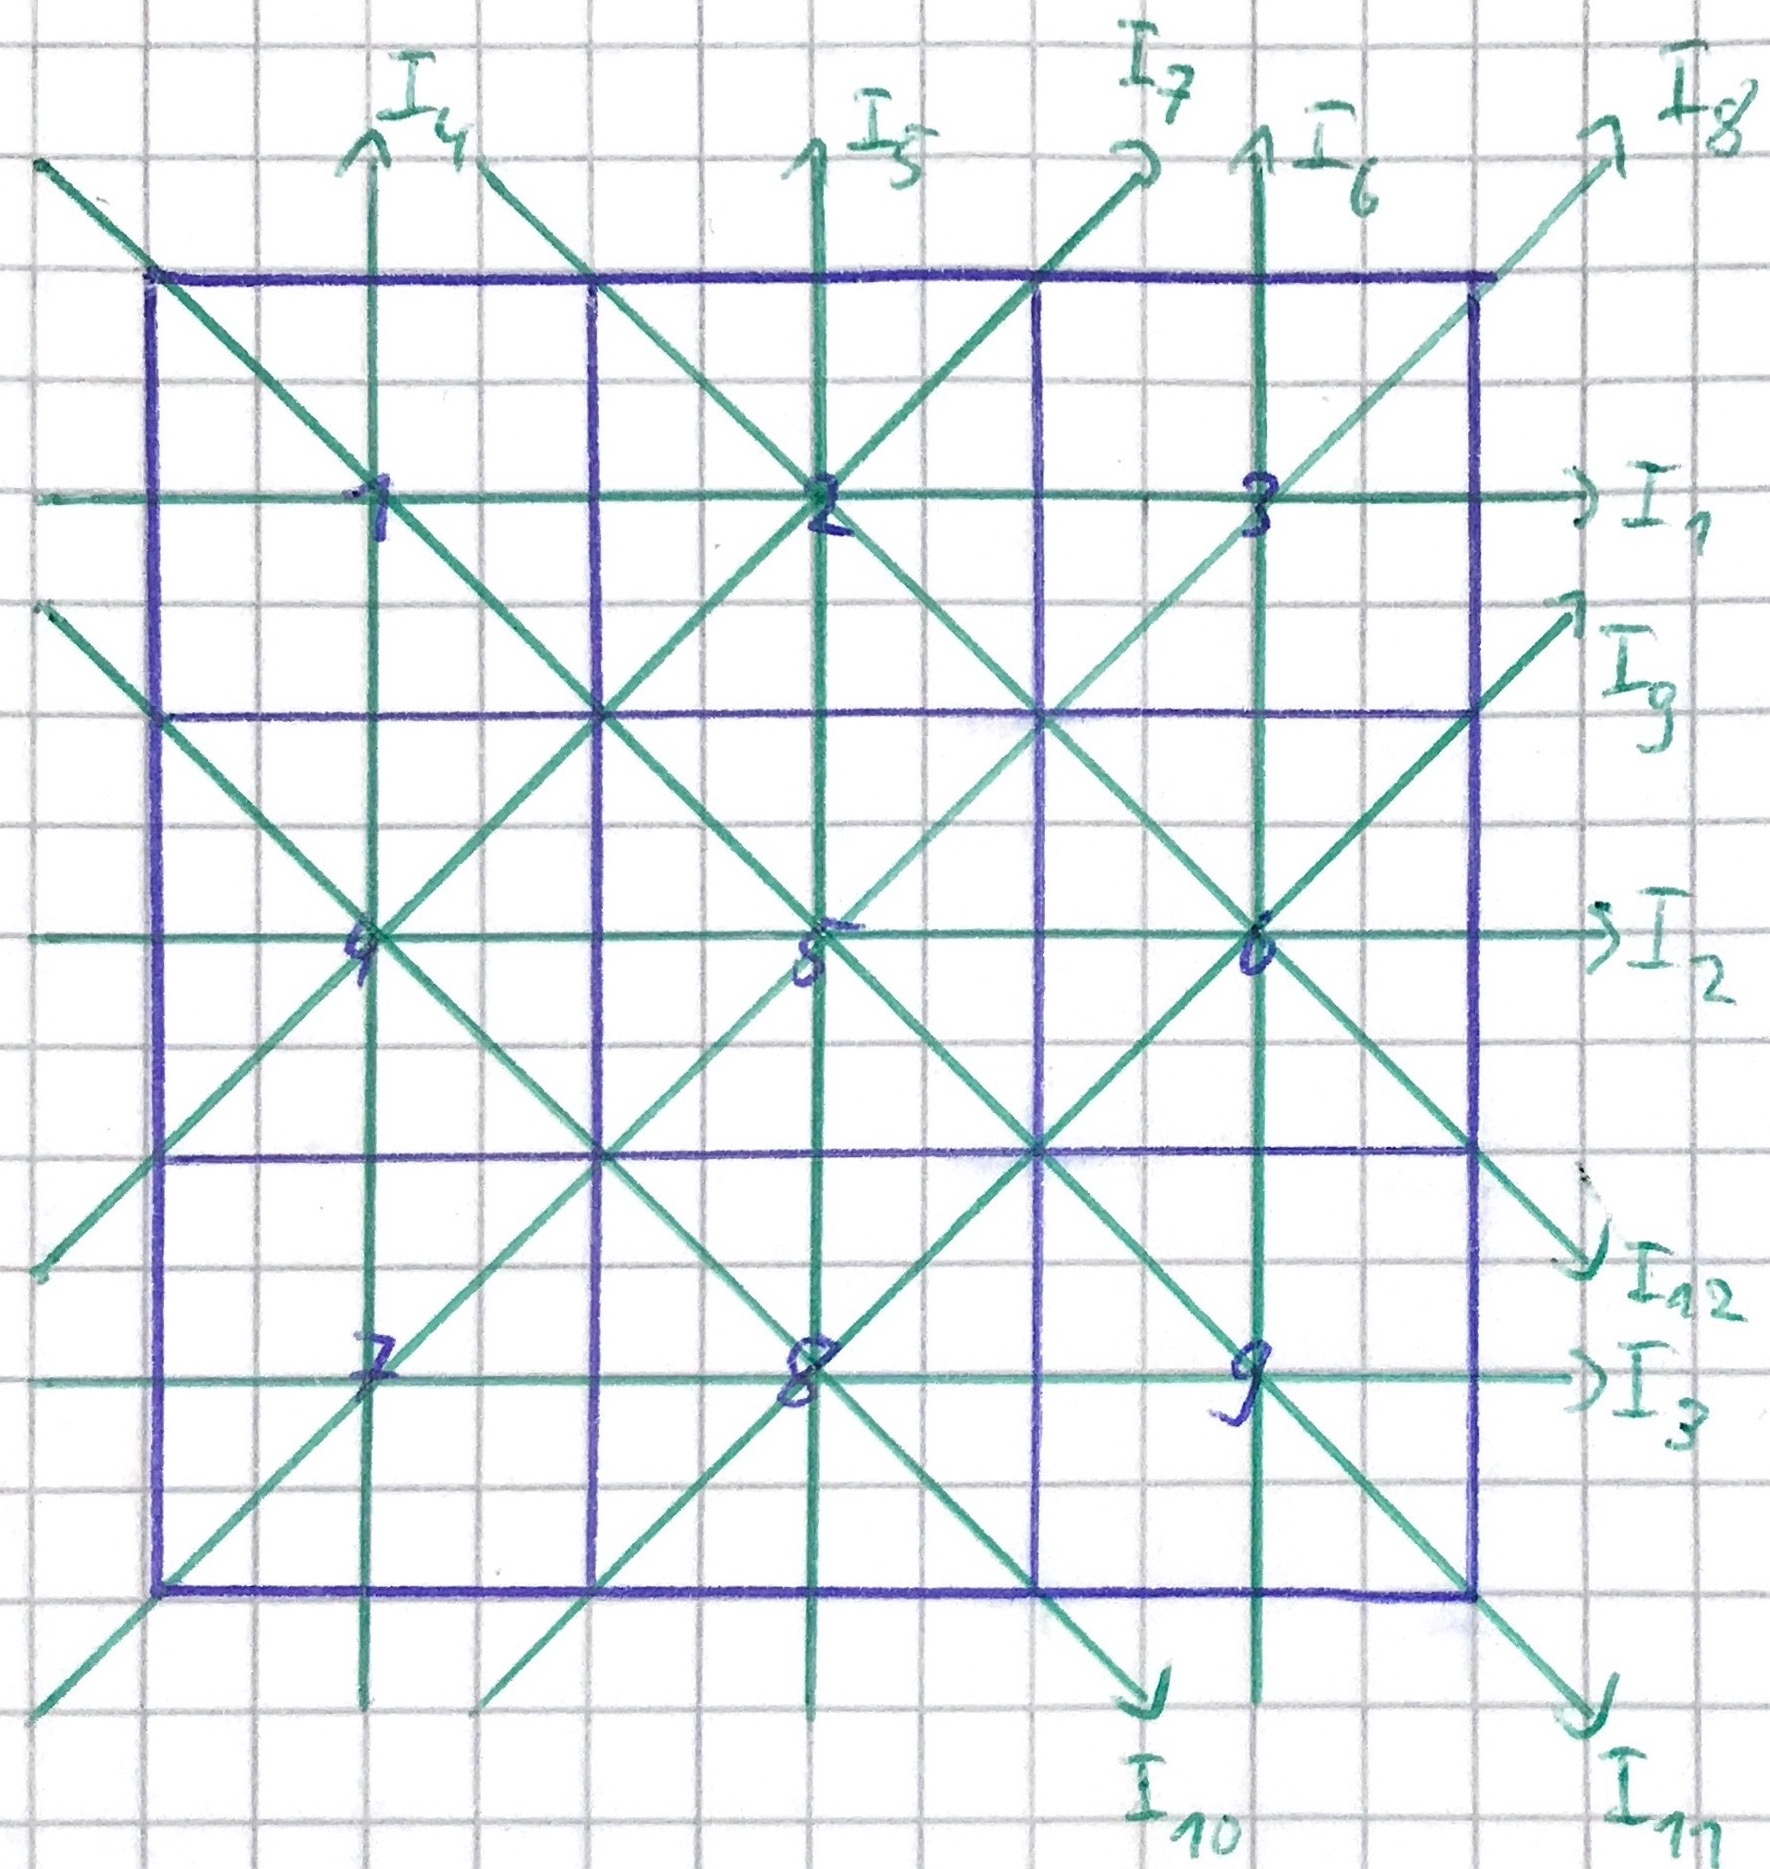
\includegraphics[width=\textwidth]{images/wuerfel4.jpg}
  \caption{Skizze der gemessenen Projektionen für den zusammengesetzten Würfel.}
  \label{fig:wuerfel4}
\end{figure}

\begin{table}[htp]
	\begin{center}
    \caption{Messwerte für die verschiedenen gemessenen Projektionen, sowie die daraus berechnete
    Zählrate.}
    \label{tab:wuerfel4}
		\begin{tabular}{ccccc}
		\toprule
			{Projektion} &{$N_4$}  & {$I_4$/(1/s)} \\
			\midrule
			1 & 10544 \pm 134 &  58,58 \pm 0,74\\
			2 &  7572 \pm 133 &  42,07 \pm 0,74\\
			3 & 10487 \pm 134 &  58,26 \pm 0,74\\
			4 & 12869 \pm 131 &  71,49 \pm 0,73\\
			5 & 13396 \pm 130 &  74,42 \pm 0,72\\
			6 & 13328 \pm 131 &  74,04 \pm 0,73\\
			7 & 11420 \pm 137 &  63,44 \pm 0,76\\
			8 &  4565 \pm  79 &  25,36 \pm 0,44\\
			9 & 20651 \pm 162 & 114,73 \pm 0,90\\
			10 & 18717 \pm 154 & 103,98 \pm 0,86\\
			11 & 12013 \pm 124 &  66,74 \pm 0,69\\
			12 & 18251 \pm 152 & 101,39 \pm 0,84\\
		\bottomrule
		\end{tabular}
	\end{center}
\end{table}

Die zugehörige Matrix lautet dann
\begin{equation}
  A= d
  \left(
  \begin{array}{rrrrrrrrr}
    1 & 1 & 1 & 0 & 0 & 0 & 0 & 0 & 0 \\
    0 & 0 & 0 & 1 & 1 & 1 & 0 & 0 & 0 \\
    0 & 0 & 0 & 0 & 0 & 0 & 1 & 1 & 1 \\
    1 & 0 & 0 & 1 & 0 & 0 & 1 & 0 & 0 \\
    0 & 1 & 0 & 0 & 1 & 0 & 0 & 1 & 0 \\
    0 & 0 & 1 & 0 & 0 & 1 & 0 & 0 & 1 \\
    0 & \sqrt{2} & 0 & \sqrt{2} & 0 & 0 & 0 & 0 & 0 \\
    0 & 0 & \sqrt{2} & 0 & \sqrt{2} & 0 & \sqrt{2} & 0 & 0 \\
    0 & 0 & 0 & 0 & 0 & \sqrt{2} & 0 & \sqrt{2} & 0 \\
    0 & 0 & 0 & \sqrt{2} & 0 & 0 & 0 & \sqrt{2} & 0 \\
    \sqrt{2} & 0 & 0 & 0 & \sqrt{2} & 0 & 0 & 0 & \sqrt{2} \\
    0 & \sqrt{2} & 0 & 0 & 0 & \sqrt{2} & 0 & 0 & 0 \\
  \end{array}
  \right)\,.
\end{equation}

Für die Intensitäten gilt
\begin{equation*}
  \vec{I}=   \left(
    \begin{array}{r}
      \ln\left(\frac{N_{0,1}}{N_{4,1}} \right) \\
      \ln\left(\frac{N_{0,1}}{N_{4,2}} \right) \\
      \ln\left(\frac{N_{0,1}}{N_{4,3}} \right) \\
      \ln\left(\frac{N_{0,1}}{N_{4,4}} \right) \\
      \ln\left(\frac{N_{0,1}}{N_{4,5}} \right) \\
      \ln\left(\frac{N_{0,1}}{N_{4,6}} \right) \\
      \ln\left(\frac{N_{0,2}}{N_{4,7}} \right) \\
      \ln\left(\frac{N_{0,3}}{N_{4,8}} \right) \\
      \ln\left(\frac{N_{0,2}}{N_{4,9}} \right) \\
      \ln\left(\frac{N_{0,2}}{N_{4,10}} \right) \\
      \ln\left(\frac{N_{0,3}}{N_{4,11}} \right) \\
      \ln\left(\frac{N_{0,2}}{N_{4,12}} \right) \\
    \end{array}
    \right) \,.
\end{equation*}

Nach Gleichung \eqref{eqn:mumatrix} kann dann der Vektor $\vec{\mu}$ zu
\begin{equation*}
  \vec{\mu}=
  \left(
      \begin{array}{r}
        \mu_1 \\
        \mu_2 \\
        \mu_3 \\
        \mu_4 \\
        \mu_5 \\
        \mu_6 \\
        \mu_7 \\
        \mu_8 \\
        \mu_9 \\
      \end{array}
      \right)=
  \left(
      \begin{array}{r}
        \SI{0.014}{1\per\centi\metre} \\
        \SI{0.099}{1\per\centi\metre} \\
        \SI{0.156}{1\per\centi\metre} \\
        \SI{0.135}{1\per\centi\metre} \\
        \SI{0.143}{1\per\centi\metre} \\
        \SI{0.068}{1\per\centi\metre} \\
        \SI{0.166}{1\per\centi\metre} \\
        \SI{0.027}{1\per\centi\metre} \\
        \SI{0.079}{1\per\centi\metre} \\
      \end{array}
      \right)
\end{equation*}
berechnet werden.

(FEHLER NOCH BERECHNEN!!!)

So können die Materialien kleinen Würfeln, aus denen die Ebene des Würfels zusammengesetzt ist, bestimmt werden. Die Zuordnungen und die Abweichungen der Werte von den Literaturwerten ist in Tabelle \ref{tab:ergebnisse2} aufgeführt.


\begin{table}[htp]
	\begin{center}
    \caption{Zuordnung der Materialien zu den Würfeln.}
    \label{tab:ergebnisse2}
		\begin{tabular}{ccc}
		\toprule
			{Würfel} & {Material}  & {Abweichung} \\
			\midrule
			1 &  & \\
			2 &  & \\
			3 &  & \\
			4 &  & \\
			5 &  & \\
			6 &  & \\
			7 &  & \\
			8 &  & \\
			9 &  & \\
		\bottomrule
		\end{tabular}
	\end{center}
\end{table}
